\section{Modelare SPICE}

\subsection{Alegerea coeficientului sursei}
Prin calcul am ajuns la coeficientul sursei de curent comandate in curent de $-3$, schema circuitului este in Fig.\ref{fig:circgay1}
Numerele nodurilor sunt aceleasi ca in graficele de curenti si de tensiune.

\begin{figure}
\begin{center}
\begin{circuitikz}[scale=1.4,european resistors,american inductors]
\draw (2,0) -- (0,0) to [R, l = $R_3$, -*] (0,4) to[R, l = $R_1$, -*] (4,4);
\draw (4,0) to[romanianCCS, l = $F_4$] (4, 4);
\draw (4,0) -- (2,0) to[romanianVoltageSource, l = $E_5$, *-] (0,4);
\draw (2,0) to [R, l = $R_2$] (4,4);
\end{circuitikz}
\caption{$R_1 = 0.5\Omega, R_2 = 2\Omega, R_3 = 1\Omega, E_5 = 1V, J_4 = 3A$}
\label{fig:circgay1}
\end{center}
\end{figure}

\begin{figure}
\begin{center}
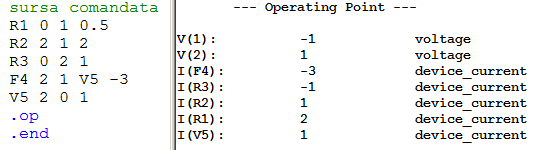
\includegraphics[width=0.6\textwidth]{spice.PNG}
\caption{grafic $I(R)$}
\end{center}
\end{figure}